\documentclass[sensors,article,submit,moreauthors, xelatex]{Definitions/mdpi} 

%=================================================================
\firstpage{1} 
\makeatletter 
\setcounter{page}{\@firstpage} 
\makeatother
\pubvolume{xx}
\issuenum{1}
\articlenumber{5}
\pubyear{2019}
\copyrightyear{2019}
%\externaleditor{Academic Editor: name}
\history{Received: date; Accepted: date; Published: date}
%\updates{yes} % If there is an update available, un-comment this line

%% MDPI internal command: uncomment if new journal that already uses continuous page numbers 
%\continuouspages{yes}

%------------------------------------------------------------------
% The following line should be uncommented if the LaTeX file is uploaded to arXiv.org
%\pdfoutput=1

%=================================================================
% Add packages and commands here. The following packages are loaded in our class file: fontenc, calc, indentfirst, fancyhdr, graphicx, lastpage, ifthen, lineno, float, amsmath, setspace, enumitem, mathpazo, booktabs, titlesec, etoolbox, amsthm, hyphenat, natbib, hyperref, footmisc, geometry, caption, url, mdframed, tabto, soul, multirow, microtype, tikz
\usepackage{biblatex}
\addbibresource{myzotero.bib}
\usepackage[acronym, nogroupskip, nonumberlist]{glossaries}

\setglossarystyle{long}
\renewenvironment{theglossary}%
  {\begin{longtable}[l]{l l p{\glsdescwidth}}}
  {\end{longtable}}
 
\makenoidxglossaries
\newacronym{roi}{ROI}{region of interest}
\newacronym{sfm}{SfM-MVS}{structure-from-motion multi-view stereo photogrammetry}
\newacronym{dom}{DOM}{digital orthophoto map}
\newacronym{dsm}{DSM}{digital surface model}
\newacronym{lidar}{LiDAR}{light detection and ranging}
\newacronym{ml}{ML}{machine learning}
\newacronym{dl}{DL}{deep learning}
\newacronym{pcd}{PCD}{point cloud data}
\newacronym{gis}{GIS}{geographic information system}
\newacronym{gcp}{GCPs}{ground control points}
\newacronym{mtp}{MTPs}{manual tie points}
\newacronym{mkl}{MKL}{math kernel library}

%=================================================================
%% Please use the following mathematics environments: Theorem, Lemma, Corollary, Proposition, Characterization, Property, Problem, Example, ExamplesandDefinitions, Hypothesis, Remark, Definition, Notation, Assumption
%% For proofs, please use the proof environment (the amsthm package is loaded by the MDPI class).

%=================================================================
% Full title of the paper (Capitalized)
\Title{EasyRIC: A post process tool for }

% Author Orchid ID: enter ID or remove command
\newcommand{\orcidauthorA}{0000-0001-6135-402X} % Add \orcidA{} behind the author's name
%\newcommand{\orcidauthorB}{0000-0000-000-000X} % Add \orcidB{} behind the author's name

% Authors, for the paper (add full first names)
\Author{Haozhou Wang $^{1}$\orcidA{} and Wei Guo $^{1}$*}
% special signal: \dagger,\ddagger in $$ parts

% Authors, for metadata in PDF
\AuthorNames{Haozhou Wang and Wei Guo}

% Affiliations / Addresses (Add [1] after \address if there is only one affiliation.)
\address[1]{
%$^{1}$ \quad Affiliation 1; e-mail@e-mail.com\\
%$^{2}$ \quad Affiliation 2; e-mail@e-mail.com
$^{1}$ \quad International Field Phenomics Research Laboratory, Institute for Sustainable Agro-ecosystem Services, Graduate School of Agricultural and Life Science, The Univerisity of Tokyo, Japan.
}

% Contact information of the corresponding author
\corres{Correspondence: guowei@g.ecc.u-tokyo.ac.jp}%; Tel.: (optional; include country code; if there are multiple corresponding authors, add author initials) +xx-xxxx-xxx-xxxx (F.L.)}

% Current address and/or shared authorship
%\firstnote{Current address: Affiliation 3} 
%\secondnote{These authors contributed equally to this work.}
% The commands \thirdnote{} till \eighthnote{} are available for further notes

%\simplesumm{} % Simple summary

%\conference{} % An extended version of a conference paper

% Abstract (Do not insert blank lines, i.e. \\) 
\abstract{Applying high-throughput phenotyping technologies in agriculture provides an advanced and efficient method for managing and breeding crops in practical applications. Compared with device-specified remote sensing technologies (laser scanning, \acrfull*{lidar}, etc.), \acrfull*{sfm}, applicable to price friendly RGB digital cameras, has been widely spread use around the world, and many commercial and open-source software are available to implement this task. However, producing good quality of its products, such as \acrfull*{dom}, \acrfull*{dsm}, and point clouds, is quite computation intensive and hard to meet the same precision of original photos. Hence, linking low computation time produced low quality \acrshort*{sfm} products back to original digital images has significant potential to improve the efficiency and precision for data processing, but to the best of our knowledge, no easy-to-use open source tool is available for this object. In this study, a pure python package called EasyRIC (easy reconstruction image converter) was developed to link original photos to \acrshort*{sfm} products. The Lotus (\textit{Nelumbo nucifera}) breeding field were used as a show case to demonstrate the following functions: 1) Clipping the \acrfull*{roi} from point clouds and compare them throught time series. 2) Clipping the \acrshort*{roi} from \acrshort*{sfm} products to raw images. 3) Generate bunch of training data in raw images from a few manual marked \acrshort*{roi}. This python package shows the great potential to integrate the high-quality original images with \acrshort*{sfm} produced products. The quick produced low quality products are also acceptable which saved plenty computation time. Also this tool can be used to generate bunch of training data for machine learning with a few manual operation.}

% Keywords
\keyword{3D reconstruction, Orthomosaic, Training data generation, Phenotyping, Open source, Pix4D}

%+++++++++++++++++++++++++++++++++++++++++++++++++++++++++

\begin{document}

\section{Introduction}
Para1: Agricultural crisis -> demand for high-throughput phenotyping

Para2: Common high-throughput phenotyping technologies -> why RGB SfM

Para3: SfM background, \textbf{algorithm}, and software (computation intensive drawbacks, need low quality to save time)

Para4: Data processing (the difficulties to of use the result of SfM, e.g. 1) low quality of DOM make canopy cover, organ detection. -> link to raw image; 2) 3D analysis not easy (require large RAM and good computation to processing point cloud, and the quality of point cloud couldn't too large -> 3D to 2d, 3D clipping, there is no common tool to make this transfer easy)

%Pix4D OpenSFM, FieldReconst (http://cse.naro.affrc.go.jp/rsugiura/FieldReconst/) introduction

Para5: 4D time series analysis demand and point cloud clipping

Para6: Training Data crisis

Para7: Objectives

\section{Methods and Materials}

This study proposed a method and implement a python package to cropping \acrshort*{sfm} software (e.g. Pix4D Mapper) produced products based on \acrfull*{roi} and linking them on original images. The functions of this packages can be clustered into three parts corresponding to three stages of 3D reconstruction: 1) SfM stage linking to "2D to 2D"; 2) MVS stage linking to "3D to 2D"; and 3) Building GIS products stage linking to "2.5D to 2D".

\subsection{Field experiment and image collection}

To obtain the materials for package developing and testing, a lotus (\textit{Nelumbo nucifera}) experimental plot in Nishi-Tokyo, Tokyo, Japan was used as a case study (Figure \ref{fig:map}.a). The total 112 different varieties of lotus were sown in squire cultivation ponds on the ???, 2017 (Figure \ref{fig:map}.b). The ordinary local management practices were used to managed all trails.

\begin{figure}[H]
  \centering
  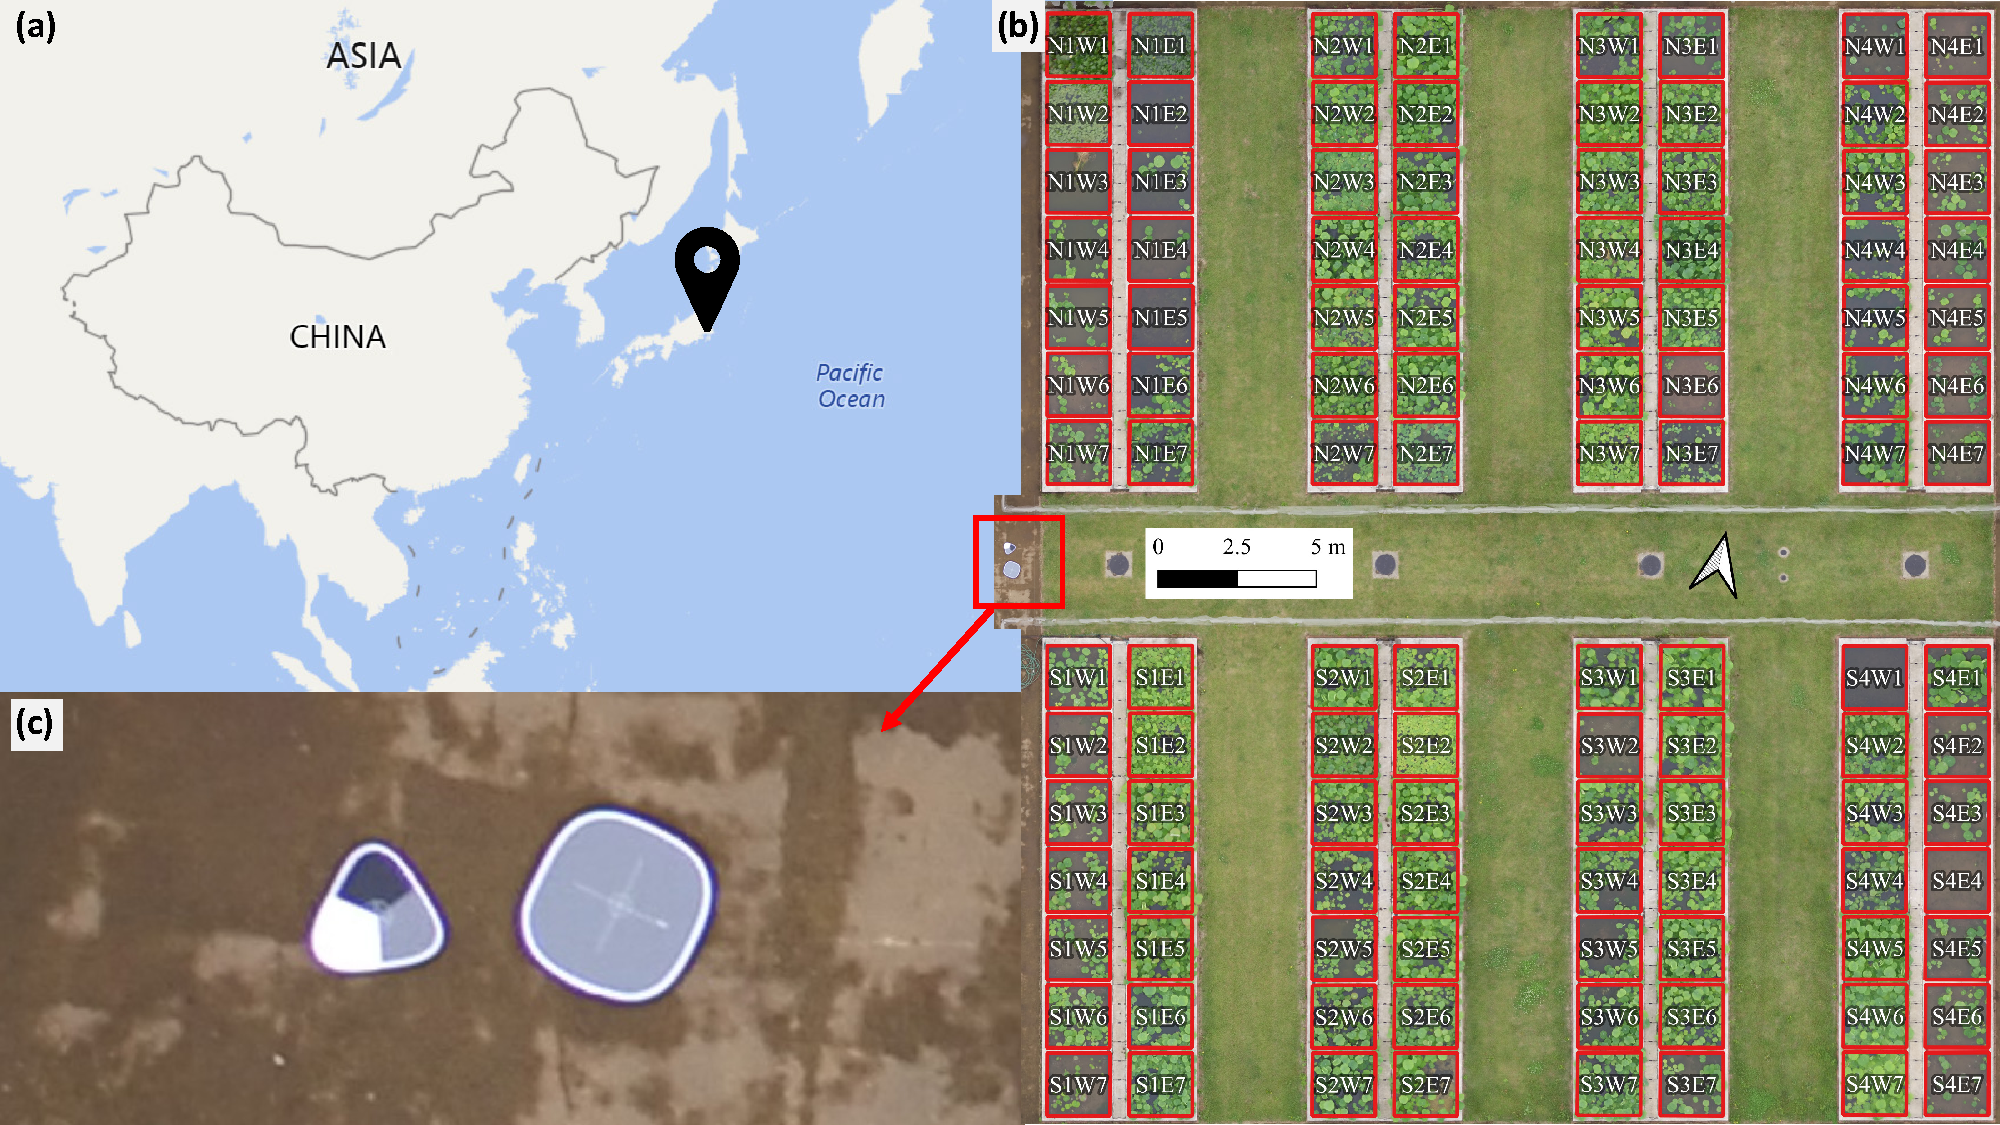
\includegraphics[width=0.95\linewidth]{figures/map.pdf}
  \caption{The experimental lotus plot condition. (\textbf{a}) the experimental plot locates in Nishi-Tokyo, Tokyo, Japan; (\textbf{b}) The labels of cultivation ponds, the orthomosaic showed here was collected on the May 5, 2017. The labels and boundaries of ponds were made by QGIS software and saved to shapefile (\*.shp) for later usage; (\textbf{c}) shows the device used for obtaining geographic position and functioning as ground control point to linking different flight time series together}
  \label{fig:map}
\end{figure}

The DJI FC550 drone (VC Technology, UK) was used to acquire images, the flight height is 30 m and the flight speed is ??? m/s. The flight route was designed by ??? software and the heading overlap and side overlap were ??? \% and ??? \% respectively. The Pix4Dmapper Pro software (Pix4D, Lausanne, Switzerland) was used to obtain the \acrshort*{sfm} products. The parameters for all \acrshort*{sfm} steps in the software were used as default, and the \acrfull*{gcp} were marked by ??? GPS device (Figure \ref{fig:map}.c). The device for 3D reconstruction processing includes Intel Xeon E5-2690 v4 @2.60GHz CPU; 128GB RAM; two NVIDIA GeForce GTX1080Ti (Driver: 26.21.14.3186) GPUs; and Windows 10 Pro, 64-bit operating system. The details of digital data collected and produced were shown in Table \ref{tab:diginfo}.

\begin{table}[H]
  \caption{Trail field and image collection information}
  \centering
  %% \tablesize{} %% You can specify the fontsize here, e.g., \tablesize{\footnotesize}. If commented out \small will be used.
  \resizebox{\textwidth}{!}{
  \begin{tabular}{ccccccc}
    \toprule
    \textbf{Flight date}	& \textbf{No. of raw images}	& \textbf{Size of raw images} & \textbf{Size of DOM} & \textbf{Size of DSM} & \textbf{Size of PCD}  & \textbf{Processing time} \\ 
    (yyyymmdd)&     & (GB) & (MB) & (MB) & (MB) & (min)\\
    \midrule
    20170525  & 266	& 1.64 & 38.5 & 34.6 & 89.2 & 39.7 \\
    20170531	& 151 & 0.94 & 40.4 & 37.6 & 60.0 & 47.3 \\
    20170603	& 141 & 0.87 & 46.5 & 34.1 & 60.3 & 18.8 \\
    20170612	& 285 & 1.74 & 38.1 & 32.9 & 93.8 & 101.5\\
    20170616	& 136 & 0.84 & 39.1 & 33.4 & 60.1 & 11.1 \\
    20170703	& 138 & 0.88 & 36.3 & 33.2 & 58.5 & 11.0 \\
    20170707	& 132 & 0.82 & 40.7 & 32.4 & 57.1 & 10.0 \\
    20170711	& 138 & 0.86 & 41.8 & 33.4 & 57.8 & 14.4 \\
    20170718	& 135 & 0.84 & 38.5 & 35.4 & 56.9 & 10.1 \\
    20170724	& 142 & 0.90 & 34.5 & 32.9 & 59.2 & 10.3 \\
    \bottomrule
  \end{tabular}
  }
  \label{tab:diginfo}
\end{table}

\subsection{Algorithms and implementation}

The general workflow of this tool was shown in Figure \ref{fig:workflow}. There were three main parts of this workflow, including preparing 3D reconstruction outputs (Figure \ref{fig:workflow}.a), preparing corresponding \acrfull*{roi} by other tools (Figure \ref{fig:workflow}.b), and EasyRIC converting tools (Figure \ref{fig:workflow}.c). Each part had tight correspondence with 3D reconstruction workflow, and was split into (1) SfM stage, (2) MVS stage, and (3) GIS products stage respectively.

\begin{figure}[H]
  \centering
  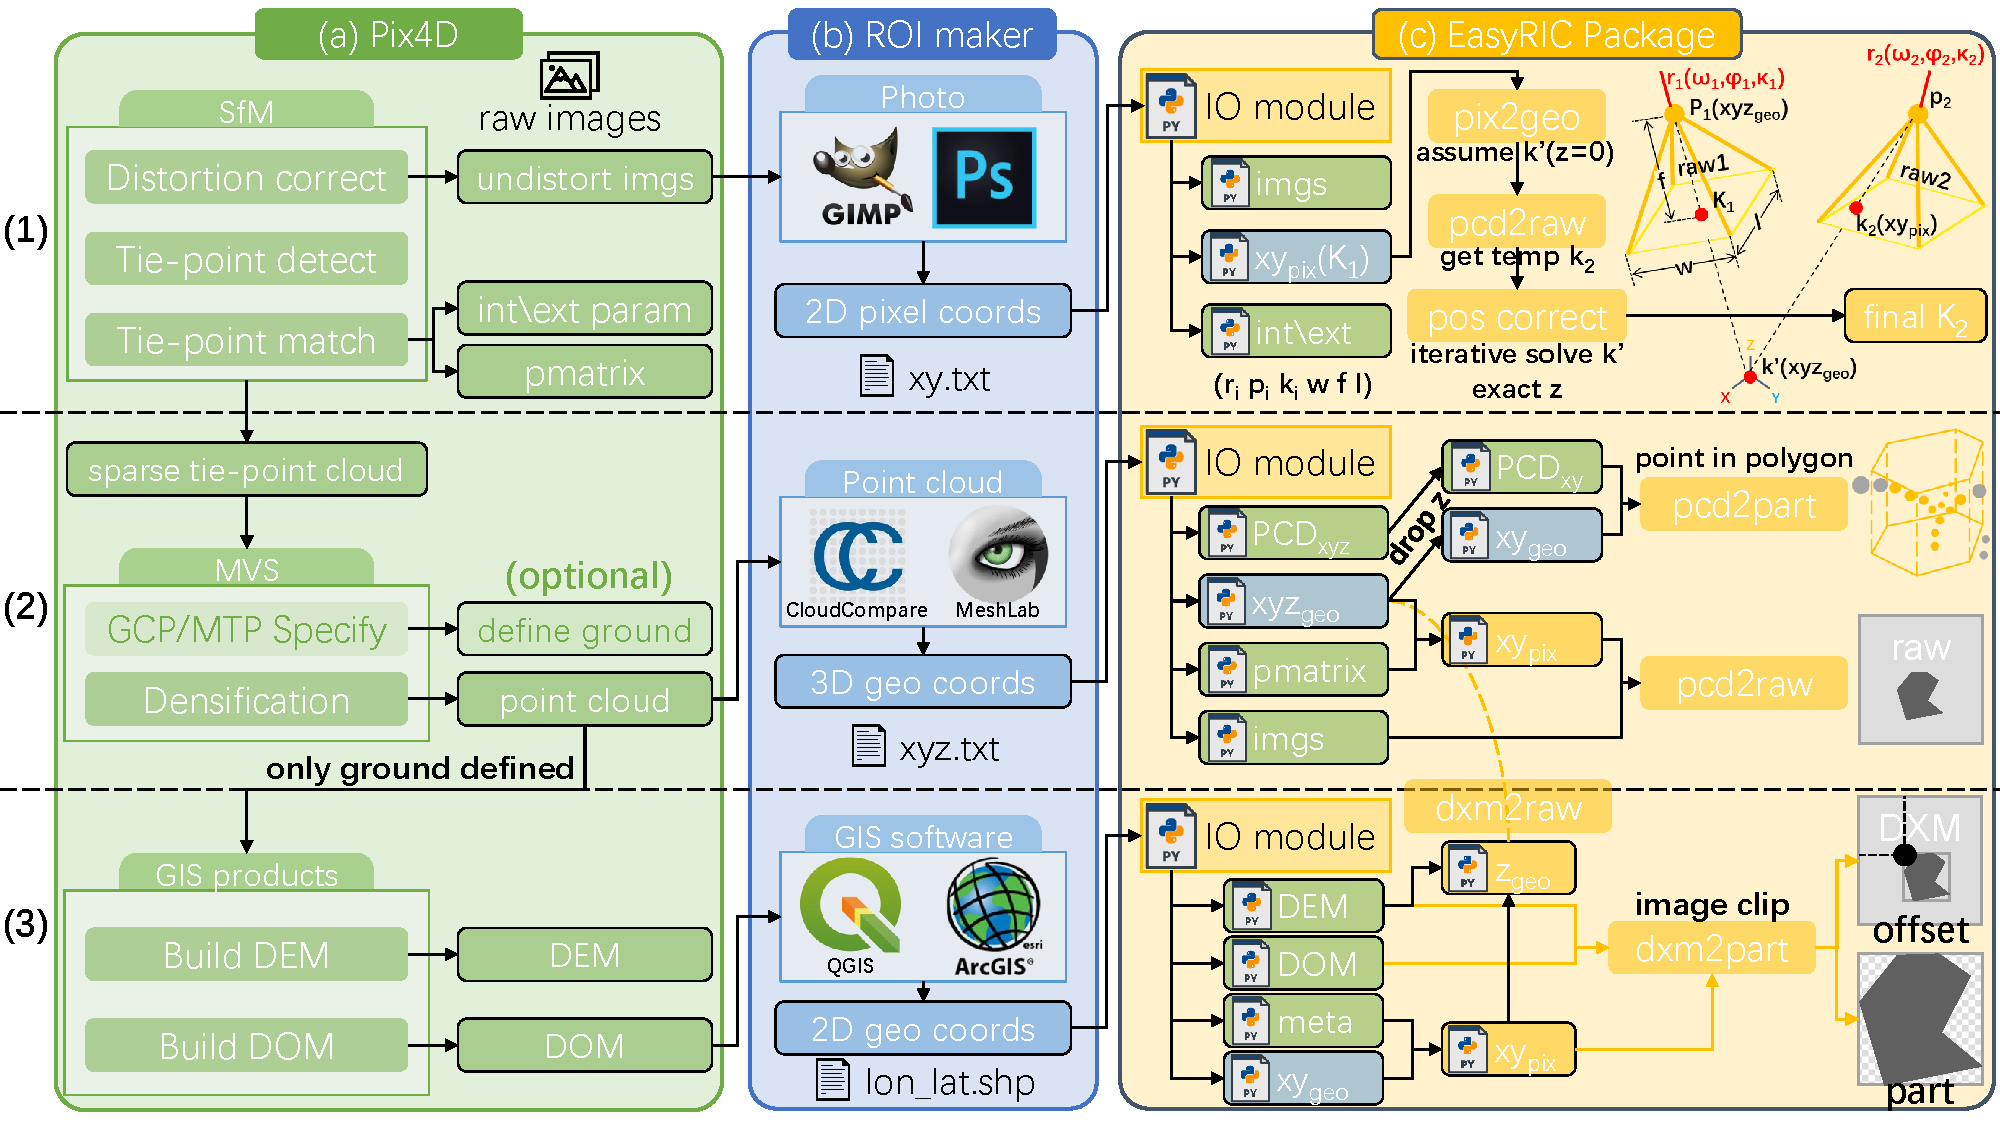
\includegraphics[width=0.95\linewidth]{figures/workflow.pdf}
  \caption{The workflow of proposed method. (\textbf{a}) The processing pipeline and output of 3D reconstruction (use Pix4Dmapper workflow as example). This step can be separated into 3 parts: (1) the structure from motion part which build the sparse tie-point cloud, the int$\setminus$ext param referred to internal and external camera parameters, and pmatrix referred to camera matrix. (2) the multi-view stereo photogrammetry part which densify previous sparse tie-point cloud and make geographic corrections based on the optional ground define step via \acrfull*{gcp} or \acrfull*{mtp}. (3) For those defined ground plots, export \acrfull*{dom} and \acrfull*{dsm}. (\textbf{b}) The \acrfull*{roi} maker pipeline via commercial or open source tools. (\textbf{c}) The processing pipeline for EasyRIC package, (1) "2D to 2D" part (ROI from image 1 to image 2), $r_i$ represented camera rotation of image $i$, $p_i$, represented camera position of image $i$, $k_i$ represented 2D pixel coordinates on image $i$, $w$ was sensor width (mm), $f$ was sensor focal length and $l$ was sensor length (mm). (2) "3D to 2D" part (ROI from point cloud data (PCD) to raw images). (3) "2.5D to 2D part" (ROI from geographic shapefile to raw images)}
  \label{fig:workflow}
\end{figure}

\subsubsection{3D reconstruction by SfM-MVS}
%The definition of each camera external parameters and 2D \& 3D coordinates

%including lens distortion correction (default FC550\_DJI camera model), automatic feature tie-points matching, manual \acrfull*{gcp} marking via ??? GPS device (Figure \ref{fig:map}.c), building densified point clouds, and exporting both \acrshort*{dom} and \acrshort*{dsm}.

%build the sparse tie-point cloud, and also produce the geometry relationship among each raw images. The geometry relationship reflects in the output files, including distortion corrected images

% miller_estimate_2015 里面有SfM-MVS的所有操作步骤



\subsubsection{Region of Interest (ROI) making}
(1) for making 2D pixel coordinates on raw or undistorted images, common photo processing software can be used, e.g. open-source GIMP or commercial Photoshop. (2) for making 3D coordinates in point cloud (or 3D geographic coordinates if ground defined), common 3D processing software can be used, e.g. CloudCompare or MeshLab. (3) for making 2D geographic polygon on DOM and DSM, common \acrfull*{gis} processing software including QGIS (open source) or ArcMap (commercial) can be used to produce required shapefiles.

\subsubsection{2D to 2D}
"2D to 2D": For those predefined ground plots, the image analyzing software (e.g. Photoshop, GIMP, etc.) was used to mark 2D pixel coordinates of \acrshort*{roi} on one original images, and calculate the 2D pixel coordinates of this \acrshort*{roi} on other original images.

\subsubsection{3D to 2D}
"3D to 2D": For both predefined and non-predefined ground plots, the \acrfull*{pcd} and point cloud analyzing software (e.g. CloudCompare) were used to obtain 3D \acrshort*{roi} directly, and the same reverse calculation as previous class was applied afterwards. The details of this method, algorithms and testing experimental plots were given below.

...(dxm2raw, extract height from DSM and obtain 3D geographic coordinates of pcd2raw) and clipping DOM and DSM by ROI (dxm2part).

\subsubsection{2.5D to 2D}
"2.5D to 2D": For those predefined ground plots, the DOM and \acrfull*{gis} software were used to produce 2D \acrshort*{roi} polygon shapefile (*.shp), and the DSM was used to obtain the height (Z axis) values in order to get the 3D coordinates of \acrshort*{roi}. Then the reverse calculation was applied to calculate the 2D pixel coordinates of this \acrshort*{roi} on given original images based on the joint rotation-translation matrix (also called camera matrix or pmatrix) produced by \acrshort*{sfm} software.

\subsubsection{Package implementation}
A open-source python \cite{guido_python_2018} package called EasyRIC (easy reconstruction image converter) was developed to implement the ideas of this paper. Though the source codes were cross-platform due to the characteristic of python language, they were programmed and tested under Windows 10 64-bit platform and Intel CPU with \acrfull*{mkl} support. For the package performance reliability, the 8GB of RAM and CPU with at 3GHz are recommended. The requirements to use this packages requires: the Python version is 3.7 or higher, and site-packages, numpy >= 1.18.1, scikit-image >= 0.16.2, opencv-python >= 3.4.2.16, pyproj==2.6.1.post1, pyparsing>=2.0.1 are required, and following pure python packages were included in source code without installation: Pyshp, Send2Trash, ezdxf, and plyfile. The user manual and source code can be accessed via: https://github.com/HowcanoeWang/EasyRIC and the License is GPL-3.0 which is free to use for any purpose, forever.

\subsection{Accuracy assessment and evaluation}
%IoU calculation and \cite{tresch_easy_2019}
\subsubsection{Intersection of union (IoU)}

\subsubsection{Time-series traits evaluation}
% calculation of coverage

% calculation of height

\section{Results}

\subsection{Use case 1: Point cloud segmentation}
Compare \acrshort*{roi} by time series

In this part, both raw photo? DOM? and point clouds should be displayed? Clipping point clouds may requires Open3D packages, which can not guarantee easy to be packed up.

\subsection{Use case 2: plot segmentation}

Find \acrshort*{roi} in \acrshort*{sfm} products on the raw images

text \cite{ma_calculation_2019, guo_illumination_2013}
should including from DOM(DSM) coordinates (GIS or pixel) and point clouds (3D) coordinates to raw images.

\subsection{Use case 3: Efficient annotation of training data for \acrshort*{ml}/\acrshort*{dl}}
3D/2.5D small region -> 2D->Raw small region, selecting strategy for efficient annotation of training data for ML/DL.

\section{Discussion}

%\subsection{Future prospects}
API for most \acrshort*{sfm} software packages

2D Photo to 2D photo without SfM products

Link between Aerial and Terrestrial photos.

\section{Conclusions}
Text

%%%%%%%%%%%%%%%%%%%%%%%%%%%%%%%%%%%%%%%%%%
\vspace{6pt} 

%\section{Availability and requirements}
%\begin{itemize}
%  \item \textbf{Project name:} EasyRIC
%  \item \textbf{Project home page:} https://github.com/HowcanoeWang/EasyRIC
%  \item \textbf{Operating system(s):} Using the source codes as Python package is platform independent, also providing executable software package for windows (windows 10 and 64-bit is tested and recommended).
%  \item \textbf{Programming language: } Python
%  \item \textbf{Other requirements:} For using source code as package: Python 3.7 or higher, numpy 1.18.1 or higher, scikit-image 0.16.2 or higher; For using executable software packages on Windows, 64-bit windows is required, and Intel CPU (with mkl support) is recommended.
%  \item \textbf{License:} GPL-3.0
%  \item \textbf{Any restrictions to use by non-academics:} Free to use for any purpose, forever.
%\end{itemize}

%%%%%%%%%%%%%%%%%%%%%%%%%%%%%%%%%%%%%%%%%%
\authorcontributions{For research articles with several authors, a short paragraph specifying their individual contributions must be provided. The following statements should be used ``conceptualization, X.X. and Y.Y.; methodology, X.X.; software, X.X.; validation, X.X., Y.Y. and Z.Z.; formal analysis, X.X.; investigation, X.X.; resources, X.X.; data curation, X.X.; writing--original draft preparation, X.X.; writing--review and editing, X.X.; visualization, X.X.; supervision, X.X.; project administration, X.X.; funding acquisition, Y.Y.'', please turn to the \href{http://img.mdpi.org/data/contributor-role-instruction.pdf}{CRediT taxonomy} for the term explanation. Authorship must be limited to those who have contributed substantially to the work reported.}

%%%%%%%%%%%%%%%%%%%%%%%%%%%%%%%%%%%%%%%%%%
\funding{Please add: ``This research received no external funding'' or ``This research was funded by NAME OF FUNDER grant number XXX.'' and  and ``The APC was funded by XXX''. Check carefully that the details given are accurate and use the standard spelling of funding agency names at \url{https://search.crossref.org/funding}, any errors may affect your future funding.}

%%%%%%%%%%%%%%%%%%%%%%%%%%%%%%%%%%%%%%%%%%
\acknowledgments{In this section you can acknowledge any support given which is not covered by the author contribution or funding sections. This may include administrative and technical support, or donations in kind (e.g., materials used for experiments).}

%%%%%%%%%%%%%%%%%%%%%%%%%%%%%%%%%%%%%%%%%%
\conflictsofinterest{Declare conflicts of interest or state ``The authors declare no conflict of interest.'' Authors must identify and declare any personal circumstances or interest that may be perceived as inappropriately influencing the representation or interpretation of reported research results. Any role of the funders in the design of the study; in the collection, analyses or interpretation of data; in the writing of the manuscript, or in the decision to publish the results must be declared in this section. If there is no role, please state ``The funders had no role in the design of the study; in the collection, analyses, or interpretation of data; in the writing of the manuscript, or in the decision to publish the results''.} 

%%%%%%%%%%%%%%%%%%%%%%%%%%%%%%%%%%%%%%%%%%
%% optional
%\abbreviations{The following abbreviations are used in this manuscript:\\

%\noindent 
%\begin{tabular}{@{}ll}
%MDPI & Multidisciplinary Digital Publishing Institute\\
%DOAJ & Directory of open access journals\\
%TLA & Three letter acronym\\
%LD & linear dichroism
%\end{tabular}}

%\renewcommand*{\glsgroupskip}{}
\printnoidxglossary[type=\acronymtype, title=Abbreviations]

%%%%%%%%%%%%%%%%%%%%%%%%%%%%%%%%%%%%%%%%%%
%% optional
%\appendixtitles{no} %Leave argument "no" if all appendix headings stay EMPTY (then no dot is printed after "Appendix A"). If the appendix sections contain a heading then change the argument to "yes".
%\appendix
%\section{}
%\unskip
%\subsection{}
%The appendix is an optional section that can contain details and data supplemental to the main text. For example, explanations of experimental details that would disrupt the flow of the main text, but nonetheless remain crucial to understanding and reproducing the research shown; figures of replicates for experiments of which representative data is shown in the main text can be added here if brief, or as Supplementary data. Mathematical proofs of results not central to the paper can be added as an appendix.

%\section{}
%All appendix sections must be cited in the main text. In the appendixes, Figures, Tables, etc. should be labeled starting with `A', e.g., Figure A1, Figure A2, etc. 

%%%%%%%%%%%%%%%%%%%%%%%%%%%%%%%%%%%%%%%%%%
% Citations and References in Supplementary files are permitted provided that they also appear in the reference list here. 
\reftitle{References}
%=====================================
% References, variant B: external bibliography
%=====================================
\externalbibliography{yes}
\bibliography{myzotero}

%%%%%%%%%%%%%%%%%%%%%%%%%%%%%%%%%%%%%%%%%%
%% optional
%\sampleavailability{Samples of the compounds ...... are available from the authors.}

%% for journal Sci
%\reviewreports{\\
%Reviewer 1 comments and authors’ response\\
%Reviewer 2 comments and authors’ response\\
%Reviewer 3 comments and authors’ response
%}

%%%%%%%%%%%%%%%%%%%%%%%%%%%%%%%%%%%%%%%%%%
\end{document}
